\usubsection{Incremento 1: Editor visual y motor de ejecución local}

El objetivo de este primer incremento fue establecer las bases funcionales del sistema, centrándose en dos componentes esenciales: el editor visual para la construcción de programas y el motor de ejecución para el procesamiento de grafos. A partir de los requerimientos definidos en la fase de análisis, se identificaron como necesidades prioritarias la capacidad de crear, conectar y ejecutar nodos dentro de un entorno web interactivo, un sistema de tipado que previniera conexiones inválidas, mecanismos de retroalimentación visual para informar al usuario sobre el estado de cada nodo durante la ejecución y un módulo de serialización que permitiera almacenar los programas construidos.

Se delimitó el alcance del incremento a la ejecución local en el navegador, postergando para iteraciones posteriores las capacidades de distribución hacia hardware externo y computadoras remotas. Se priorizó la implementación de las funcionalidades mínimas necesarias para permitir la programación visual básica, organizando el trabajo en las siguientes líneas de desarrollo:

\begin{itemize}
    \item Construcción del editor visual con su lienzo de trabajo y paleta de nodos.
    \item Motor de ejecución basado en activación por disponibilidad de datos.
    \item Catálogo inicial de nodos orientado a operaciones básicas.
    \item Módulo de exportación e importación de programas.
    \item Retroalimentación visual del estado de los nodos.
    \item Sistema de validación de tipos en las conexiones.
\end{itemize}

Se modeló una arquitectura compuesta por dos subsistemas principales: el editor visual y el intérprete del grafo. Para el editor se definió un entorno basado en la metáfora de arrastrar y soltar, con un lienzo central, una paleta lateral de nodos y un sistema de conexiones entre puertos visuales. Para el motor de ejecución se planteó un modelo de activación por disponibilidad de datos, gestionado mediante un bucle de eventos que evalúa continuamente qué nodos están listos para
ejecutarse. Este diseño contempló la posibilidad de ejecución concurrente a nivel lógico entre ramas independientes del grafo.

Adicionalmente, se diseñó un catálogo inicial de nodos que cubría operaciones de procesamiento numérico, lógico y textual. Se definió un esquema de serialización basado en un formato JSON estructurado y versionado, capaz de almacenar la versión del documento, el nombre del programa, la configuración de los nodos con sus interconexiones (de forma separada: un arreglo de nodos y un arreglo de conexiones) y los parámetros espaciales del lienzo.

Para la retroalimentación visual se diseñó una máquina de estados que representara el ciclo de vida de cada nodo mediante cuatro estados: \textit{en espera} (contorno gris), \textit{activo} (contorno azul con indicador de carga), \textit{ejecución exitosa} (contorno verde) y \textit{error} (contorno rojo con mensaje descriptivo del fallo).

Finalmente, se especificó un mecanismo de validación de tipos donde cada puerto posee un tipo de dato asociado que determina su compatibilidad, representado visualmente mediante formas geométricas únicas en los puntos de conexión.

Se procedió a la implementación de la interfaz de usuario. En este proceso fueron de gran utilidad las primitivas de la librería React Flow, que ofrece un componente de lienzo, un componente base de nodo y funciones para la gestión de conexiones. Las principales tareas realizadas fueron:

\begin{itemize}
    \item \textbf{Lienzo de trabajo:} Se desarrolló un entorno que permite seleccionar nodos desde un panel lateral y depositarlos en un área de trabajo.
    \item \textbf{Gestión de conexiones:} Se implementó la lógica para trazar arcos entre los puertos de salida de un nodo y los puertos de entrada de otro, estableciendo así el grafo de flujo de datos.
    \item \textbf{Representación visual de nodos:} Se utilizaron íconos temporales, priorizando la correcta identificación de los tipos de puertos sobre el diseño visual definitivo del lenguaje.
\end{itemize}

En paralelo, se construyó el motor de ejecución bajo un enfoque interpretado, lo cual permitió ejecutar programas de forma inmediata en el navegador y facilitó las tareas de depuración. El motor implementa el bucle de eventos descrito en el modelado: identifica nodos listos para ejecutarse, procesa su lógica y propaga sus salidas hacia los nodos subsiguientes.

Tras las primeras pruebas funcionales del editor y el motor, se identificaron oportunidades de mejora en la especificación original de los nodos, lo que llevó a ajustes en el catálogo:

\begin{itemize}
    \item \textbf{Especialización de constantes:} Se descartó el nodo genérico de ``Constante'' a favor de nodos específicos de Número, Valor lógico y Texto, reduciendo así los errores al momento de programar.
    \item \textbf{Expansión de operadores matemáticos:} Se agregaron los nodos de Resto, Piso, Techo y Redondear para aumentar la capacidad expresiva en el ámbito aritmético.
    \item \textbf{Generación de datos:} Se introdujo el nodo ``Generar pulsos'', capaz de emitir valores enteros secuenciales entre un inicio y un fin con un paso definido, fundamental para probar el comportamiento de flujos continuos como los presentes en sistemas de IoT.
\end{itemize}

Seguidamente, se implementó el módulo de serialización y deserialización de grafos. Durante la exportación, el sistema extrae el estado actual del lienzo y ejecuta una rutina de limpieza para eliminar propiedades exclusivas de la sesión activa, asegurando que el archivo resultante sea completamente portable; finalmente, se descarga el archivo JSON utilizando las capacidades nativas del navegador. Durante la importación, el sistema lee el archivo suministrado por el usuario y valida de forma estricta que la versión del documento coincida con la soportada por el motor. Si la validación
es exitosa, la rutina de deserialización genera los componentes visuales, resuelve posibles conexiones huérfanas y restaura la perspectiva del lienzo tal como fue guardada. En caso de detectar un archivo corrupto o incompatible, el proceso se interrumpe y se notifica al usuario.

La máquina de estados del ciclo de vida de los nodos se materializó mediante un controlador intermedio que intercepta los eventos emitidos por el motor y traduce las transiciones lógicas en actualizaciones visuales sobre los componentes del lienzo. Estos comportamientos se evidencian en la figura~\ref{fig:estados-ejecucion-nodos}, donde se observan de forma comparativa los estados principales durante la ejecución.

\begin{figure}[H]
    \centering
    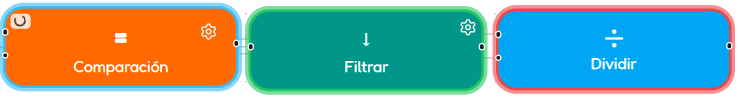
\includegraphics[width=0.5\textwidth]{../images/estados-ejecucion.png}
    \caption[Estados visuales durante la ejecución de nodos]{\normalfont Estados visuales durante la ejecución de nodos}
    \label{fig:estados-ejecucion-nodos}
\end{figure}

Finalmente, se implementó el sistema de validación de tipos en tiempo de edición. El sistema bloquea de forma activa cualquier intento de enlazar puertos con tipos incompatibles y emite mensajes descriptivos al usuario. Además, el entorno proporciona retroalimentación predictiva: al arrastrar una nueva conexión, se resaltan automáticamente los puertos de destino válidos, guiando al alumno en la construcción adecuada de su algoritmo.

Al concluir la implementación, se ejecutaron pruebas funcionales sobre programas de prueba construidos con los nodos desarrollados. Estas pruebas verificaron el correcto funcionamiento del editor, la representación visual diferenciada de tipos mediante estilos únicos y la capacidad del motor asíncrono para activar nodos automáticamente según la disponibilidad de sus entradas, procesando ramas independientes del grafo de forma lógicamente paralela.

No obstante, como parte de la evaluación pedagógica temprana, se intentó modelar algoritmos clásicos como el factorial y la sucesión de Fibonacci, evidenciando una limitación importante: la ausencia de soporte para recursividad. Este hallazgo restringió la expresividad del lenguaje para representar estructuras algorítmicas fundamentales, definiendo una línea clara de trabajo para el siguiente incremento.

Como resultado de este incremento se obtuvo una versión funcional del lenguaje capaz de ejecutar algoritmos matemáticos y lógicos dentro del navegador, sin requerir instalaciones adicionales, con retroalimentación visual continua y mecanismos de persistencia mediante serialización JSON. En la figura~\ref{fig:editor-incr1} se aprecia la interfaz en esta etapa, evidenciando la paleta de nodos, el área de diseño y la consola de salida.

\begin{figure}[H]
    \centering
    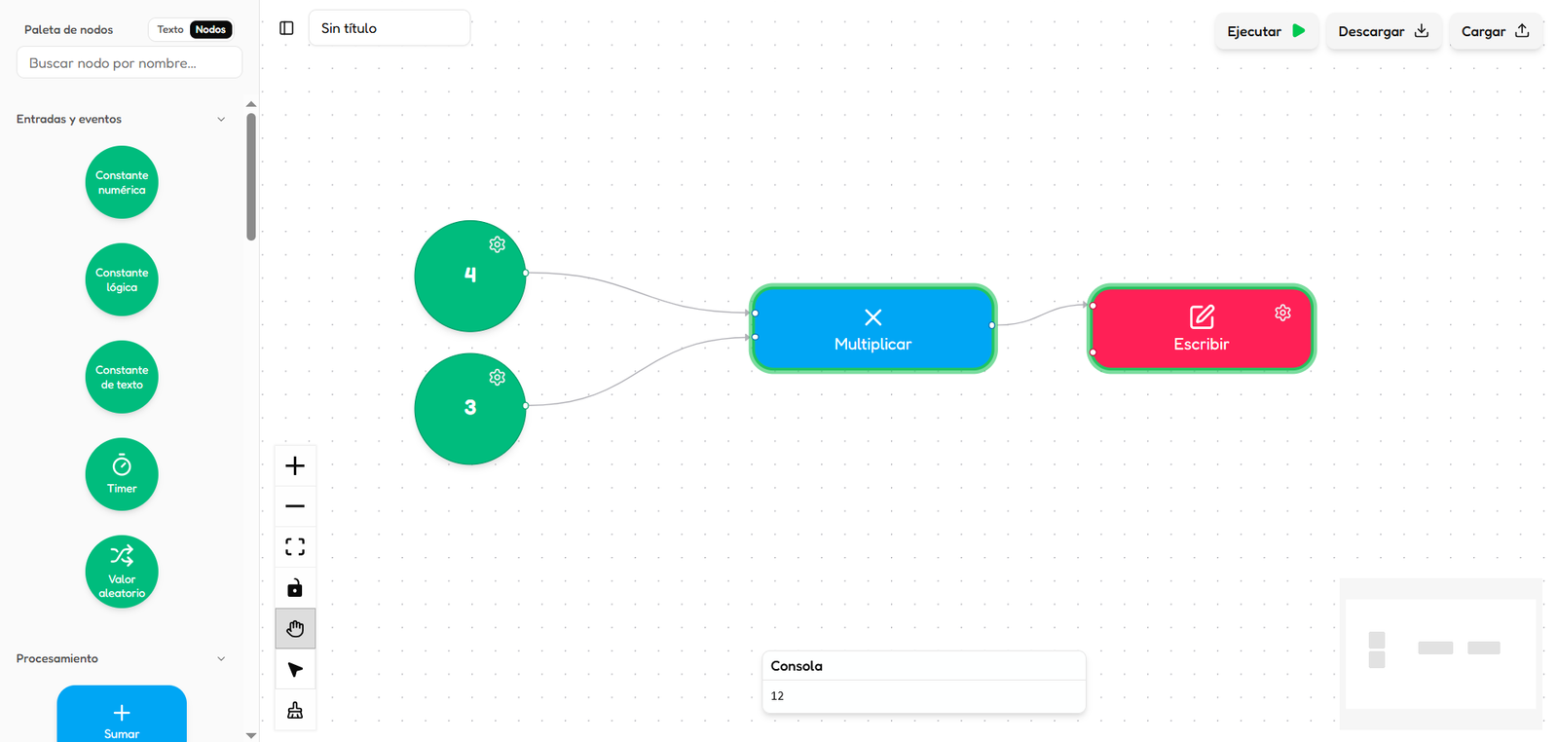
\includegraphics[width=0.85\textwidth]{../images/editor-incr1.png}
    \caption[Interfaz del editor en el primer incremento]{\normalfont Interfaz del editor en el primer incremento}
    \label{fig:editor-incr1}
\end{figure}